%\date{04.11.2008} %durch auskommentieren automatisch das aktuelle datum
\author{\labTeam}

%%%%%%%%%%%%%%%%%%%%%%%%%%%%%%%%%%%%%%%%%%%%%%%%%%%%%%%%%%%%%
% Titel
%%%%%%%%%%%%%%%%%%%%%%%%%%%%%%%%%%%%%%%%%%%%%%%%%%%%%%%%%%%%%

\title{Projekt zur GdI 1 - \labTerm}


\begin{document}
\maketitle										% Erzeugt den Titel mit Author und Datum
\centerline{Version \version}
\tableofcontents % Erzeugt das Inhaltsverzeichniss
\newpage
\setlength\parskip{0.25\baselineskip}

\section{Einführung in das Projekt}
\label{sec:intro}

Im Rahmen des Projekts implementieren die Student\_innen\footnote{Diese Schreibweise wird durchg\"angig verwendet, um alle m\"oglichen Personen gleichberechtigt anzusprechen, auch wenn sie
f\"ur den\_die Leser\_in vielleicht teilweise irritierend wirkt. Betrachten Sie dies als Reflektionsm\"oglichkeit! Mehr Informationen unter 
\url{http://de.wikipedia.org/wiki/Geschlechtergerechte_Sprache\#Sichtbarmachung} bei \glqq{}Gender Gap\grqq{}.}
in Gruppen von jeweils vier Personen eine Java-Version des Spiels \emph{\gameTitle.} Die Aufgabenstellung stellt zun\"achst das zugrundeliegende Spiel vor.

Die Aufgabe kann in vier verschiedenen \glqq Ausbaustufen\grqq\ bearbeitet werden, die jeweils eine unterschiedliche Punktzahl zur Gesamtnote beitragen. Die minimale Ausbaustufe muss zum Erreichen der Mindestpunktzahl \textbf{vollst\"andig} implementiert werden.

Ab Ausbaustufe I können nicht erreichte Punkte der gegebenen Ausbaustufe durch Elemente h\"oherer Ausbaustufen \glqq{}ausgeglichen\grqq{} werden. Projektabgaben, die \glqq{}zwischen\grqq{} Ausbaustufen liegen, bei denen also erwartete Inhalte fehlen oder zusätzliche Elemente eingebaut wurden, sind natürlich ebenfalls möglich; die Ausbaustufen geben nur eine grobe Orientierung vor. Beachten Sie dabei jedoch, dass die Ausbaustufen nach Schwierigkeitsgrad gruppiert sind, d.h.  Aufgaben h\"oherer Stufen sind in der Regel schwieriger zu l\"osen als Aufgabenteile niedrigerer Ausbaustufen.

%\newpage
\subsection{Das Spiel \emph{\gameTitle}}
 ////////////////ändern! gameIntro.tey
Im Spiel \emph{\gameTitle{}} spielen Sie Eins gegen Eins. Jede Person steuert dabei einen Gorilla und versucht den gegnerischen Gorilla mit einer Banane abzuwerfen. Die Gorillas stehen in gewisser Entfernung, einer links und einer rechts, auf verschiedenen Hochh\"ausern einer Skyline. Das Spiel ist rundenbasiert: Zun\"achst t\"atigt der/die erste Spieler\_in den Wurf. Trifft dieser Wurf, so wurde die Runde gewonnen, ansonsten ist der/die n\"achste Spieler\_in an der Reihe. Ein Wurf wird durch zwei Eingaben gesteuert: den Abwurfwinkel und die Wurfgeschwindigkeit. Der Winkel wird als Gradzahl von 0 bis 360 angegeben, die Geschwindigkeit auf einer Skala von 0 bis 200.

Abbildung \vref{fig:screenshot1} zeigt ein m\"ogliches Menü. Abbildung \vref{fig:screenshot2} zeigt ein mögliches Spielfenster. Wir erwarten nicht, dass 
das im Rahmen des Projekts erstellte Spiel der Ausgabe optisch \"ahnlich sieht; die 
Abbildung soll nur zum besseren Nachvollziehen dienen.

Auf einem beliebig großen rechteckigen Spielfeld kann es folgende Spielobjekte geben:
\begin{description}
\item[Gorilla]
Jeder Spieler verfügt über einen Gorilla. Folglich befinden sich zum Start zwei Gorillas, einer links und einer rechts, auf dem Feld. Gorillas unterschiedlicher Parteien müssen nicht visuell unterscheidbar sein.
\item[Hochhaus]
Die Gorillas stehen auf Hochhäusern, die eine Skyline bilden.
\item[Banane]
Tätigt ein Spieler einen Wurf, so fliegt eine Banane (hoffentlich) in Richtung des gegnerischen Gorillas.
\end{description}

\begin{figure}[htb]
\begin{center}
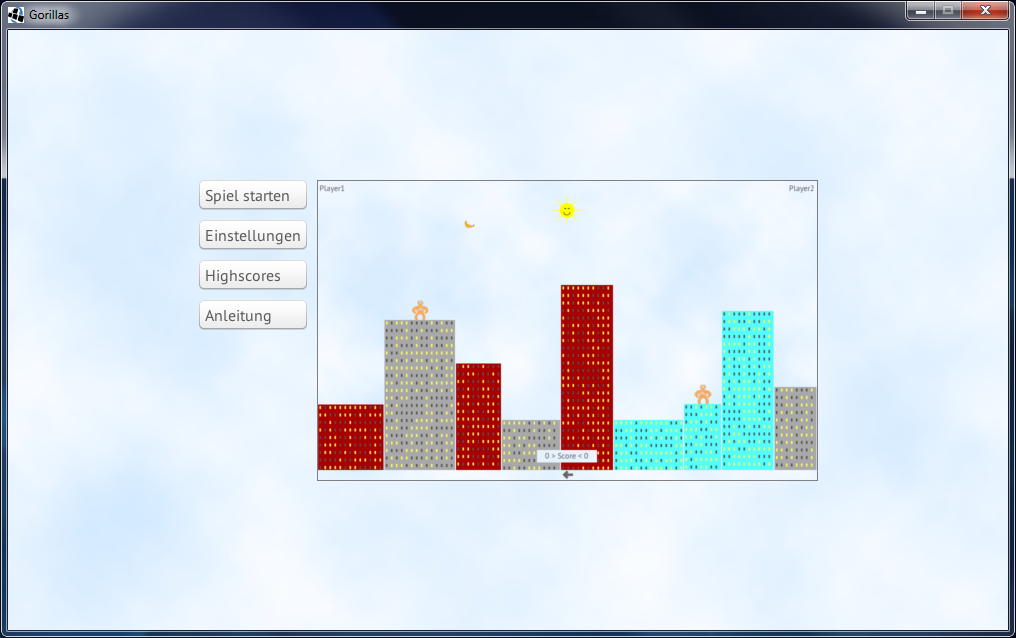
\includegraphics[scale=0.4]{\basepath/\shortGameTitle/menu.png}
\caption{Beispiel einer grafischen Umsetzung des Menüs von \gameTitle}
\label{fig:screenshot1}
\end{center}
\end{figure}

\begin{figure}[htb]
\begin{center}
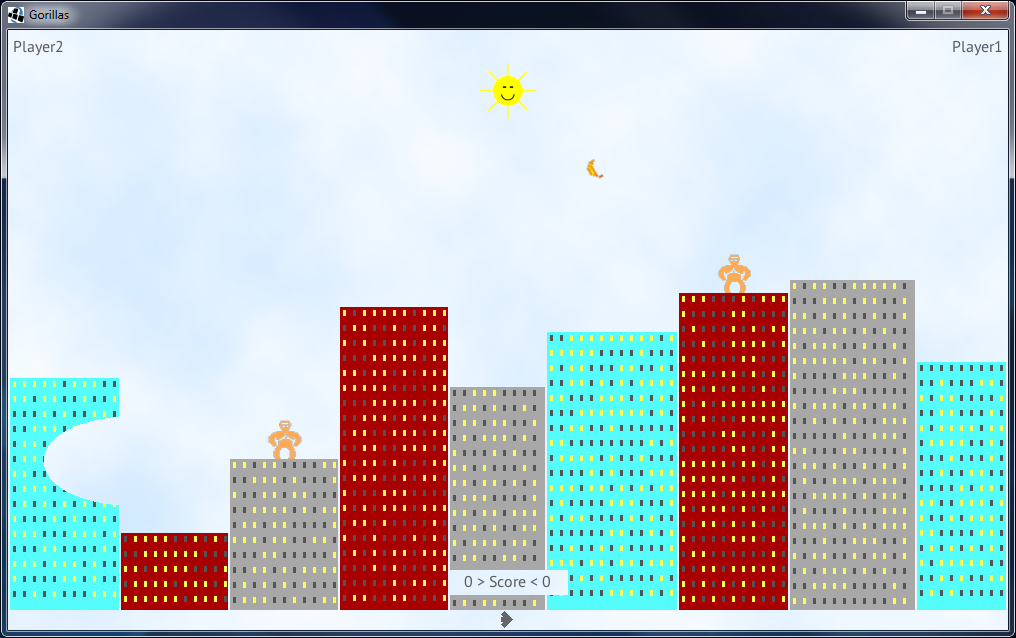
\includegraphics[scale=.4]{\basepath/\shortGameTitle/gameplay.png}
\caption{Beispiel einer grafischen Umsetzung des Spielfensters von \gameTitle}
\label{fig:screenshot2}
\end{center}
\end{figure}


\input{orga}
\section{Ihre Aufgabe}
\label{sec:aufgabe}

Implementieren Sie eine lauff\"ahige Java-Version des Spiels \emph{\gameTitle}, die
mindestens der \glqq minimalen Ausbaustufe\grqq\ entspricht. 

Das fertige Spiel muss von dem\_der Tutor\_in \emph{vor Ende des Projekts testiert werden}.
Dazu müssen die Dokumentation (etwa 2 DIN A4-Seiten) sowie der Source-Code und
alle zum Übersetzen notwendigen Bibliotheken und Dateien---au\ss{}er den von uns
im Portal bereitgestellten---rechtzeitig vor Ablauf der Einreichung \textbf{von \textit{einem} Gruppenmitglied im Portal hochgeladen werden}.

Das Testat besteht aus den folgenden drei Bestandteilen:

\begin{description}
\item[Live-Test] Der\_die Tutor\_in startet das Spiel und testet, ob alles so funktioniert wie spezifiziert.
Dazu werden potenzielle bestimmte vorgegebene Szenarien durchgespielt, aber auch
zufällig \glqq{}herumgespielt\grqq{}.

\item[Software-Test] Der\_die Tutor\_in testet die Implementierung mit den für alle
Teilnehmer\_innen bereitgestellten (\"offentlichen) und nur f\"ur die Tutor\_innen und
Mitarbeiter\_innen verf\"ugbaren (privaten) JUnit-Tests. Alle Tests m\"ussen
\textbf{ohne Benutzerinteraktion} abgeschlossen werden k\"onnen.

\item[Code-Review] Der\_die Tutor\_in sieht sich den Quellcode sowie die Dokumentation an
und stellt Fragen dazu.
\end{description}


\subsection{Ablauf des Code-Review}
\label{sec:codeReview}

Im Hinblick auf den Code-Review sollten Sie auf gut verst\"andlichen und
dokumentierten Code sowie eine sinnvolle Klassenhierarchie achten, in der Regel
auch mit Aufteilung der Klassen in Packages.

Der\_die Tutor\_in wird einzelne Gruppenmitglieder seiner Wahl zu Teilen des Quelltexts befragen.
Daher sollte sich jedes Gruppenmitglied mit allen Codeteilen auskennen---der\_die Tutor\_in
w\"ahlt aus, zu \emph{welchem Thema} eine Frage gestellt wird und w\"ahlt auch aus, \emph{wer}
die Frage beantworten soll. Die Bewertung dieses Teils bezieht sich also auf die
Aussage eines \glqq{}zuf\"allig ausgew\"ahlten\grqq{} Gruppenmitglieds, geht
aber in die Gesamtpunktzahl der Gruppe ein. 

Damit soll einerseits die \glqq{}Trittbrettfahrerei\grqq{} reduziert werden (\glqq{}ich habe
zwar nichts getan, will aber dennoch die Punkte haben\grqq{}). Gleichzeitig f\"ordert
diese Regelung die Gruppenarbeit, da auch und gerade besonders \glqq{}starke\grqq{}
Mitglieder verst\"arkt R\"ucksicht auf \glqq{}schw\"achere\grqq{} nehmen 
m\"ussen---sonst riskieren sie eine schlechtere Punktzahl, wenn \glqq{}der\_die Falsche\grqq{}
gefragt wird. Durch eine entsprechend bessere Abstimmung in der Gruppe steigen
die Lernm\"oglichkeiten \textbf{aller} Gruppenteilnehmer. Auch für (vermeintliche?)
\glqq{}Expert\_innen\grqq{} wird durch das Nachdenken \"uber die Frage \glqq{}wie erkläre ich das verst\"andlich?\grqq{} das eigene Verst\"andnis vertieft.

\subsection{Dokumentation}
\label{sec:docu}

Neben dem Quelltexten ist auch eine kurze Dokumentation abzugeben (etwa 2 DIN
A4-Seiten). Diese sollte die \emph{Klassenstruktur} ihrer L\"osung in UML umfassen und kurz auf die in ihrer Gruppe \emph{aufgetretenen Probleme} eingehen
sowie \emph{Feedback zur Aufgabenstellung} liefern. Nur die Klassenstruktur geht
in die Bewertung ein; die anderen Elemente helfen uns aber dabei, das Projekt
in der Zukunft besser zu gestalten und sind daher f\"ur uns sehr wichtig. Sie k\"onnen den Teil mit der (hoffentlich konstruktiven) 
Kritik am Projekt auch gerne separat auf Papier---auf Wunsch ohne Angabe des Gruppennamens---dem\_der Tutor\_in geben, wenn Sie das Feedback lieber anonym geben wollen.

Für die Erstellung der Klassendiagramme können Sie beispielsweise die folgenden Tools nutzen:

\begin{itemize}
\item \emph{doxygen} (\url{https://www.doxygen.nl}) ist eine Alternative
zu JavaDoc, die---bei Wahl der entsprechenden Optionen---auch Klassendiagramme
erzeugt. Eine Dokumentation zu \emph{doxygen} finden Sie auf der
obenstehenden Projekt-Homepage.

\item \emph{Fujaba} (\url{https://web.cs.upb.de/archive/fujaba})

\item \emph{BlueJ} (\url{https://bluej.org/})
\end{itemize}

Dies sind nur unsere Empfehlungen. Es steht Ihnen selbstverst\"andlich frei,
andere Tools zu nutzen, etwa OpenOffice Draw oder Microsoft Word. Bitte reichen Sie
die Dokumentation und insbesondere das Klassendiagramm als \textbf{PDF-Datei} ein.

\textbf{Zus\"atzlich} sind mindestens \emph{vier} repr\"asentative Screenshots Ihres Spiels einzureichen, darunter ein Bild vom Startmen\"u.

\subsection{Hinweise}
\label{sec:hinweise}

Denken Sie bitte daran, dass \textbf{Testf\"alle keine Interaktion mit den Spieler\_innen erfordern d\"urfen}.

Sollten Sie sich für die Nutzung des vorgegebenen Frameworks entscheiden, so nutzen Sie das Konzept von Entitäten, Ereignissen und Aktionen. Die Tutor\_innen werden bewerten, wie gut Ihnen das gelungen ist.

Sollten Sie nicht das vorgegebene Framework verwenden, so sollten Sie in Ihrem Code strikt zwischen Logik (Code) und Darstellung (Design) unterscheiden. Die Tutor\_innen werden bewerten, wie gut diese Trennung bei Ihnen gelungen ist.


\input{minimal} % Minimale Ausbaustufe
\input{ausbau1} % Ausbaustufe 1
\input{ausbau2} % Ausbaustufe 2
\input{ausbau3} % Ausbaustufe 3
\input{bonuspunkte} % Zusatz-Bonuspunkte

\input{\shortGameTitle/format} % dateiformat

\section{Materialien}

Auf der Veranstaltungsseite stellen wir Ihnen einige Dateien zur Verf\"ugung, die Sie f\"ur Ihre L\"osung verwenden k\"onnen. Dabei handelt es sich um vorgefertigte Karten und
die \"offentlichen Testf\"alle. Es wird Ihnen dringend nahe gelegt, auch unser bereitgestelltes Framework nutzen. Das Framework ist threadsicher!

\textbf{Hinweis:} Sie dürfen auch eine vollst\"andig eigene L\"osungen implementieren. Der dadurch entstehende Mehraufwand wird aber nicht durch Punkte gewürdigt. Ihre L\"osung \textbf{muss} in jedem Fall mit den bereitgestellten Testklassen \"uberpr\"ufbar sein.

Neben der kurzen Beschreibung in diesem Dokument gibt Ihnen die
JavaDoc-Dokumentation n\"utzliche Hinweise zur Verwendung und den
Parametern der vorhandenen Funktionen. Ein Blick in diese Quellen empfiehlt sich
sehr---\textbf{am besten vor dem Gang zum\_zur Tutor\_in}, um$\ldots$

\begin{itemize}
\item sich selbst und auch dem\_der Tutor\_in wertvolle Zeit zu sparen, da sich so unter Umst\"anden banale Fragen von selbst l\"osen,

\item Nerven zu sparen, da das Warten auf die Antwort der Tutor\_innen Ihre Nerven beanspruchen wird :-),

\item sich selbstst\"andiges Arbeiten anzueignen.
\end{itemize} 


\subsection{Klasse \emph{de.tu\_darmstadt.informatik.fop.gorillas.main.Gorillas}}

\textit{\gameTitle} erbt von \textit{org.slick.StateBasedGame}. \textit{\gameTitle} dient sowohl als Container für Spiele 
als auch zum Starten des gesamten Spiels. Sie müssen diese Klasse erweitern, um zusätzliche States hinzuzufügen. Lesen Sie sich dazu das \tutorialURL durch.

\subsection {Die ersten Schritte}
Sie sollten sich zunächst das  \tutorialURL 
durchlesen, um das Konzept des Frameworks zu verstehen. Anschließend können Sie in \texttt{\gameTitle} zusätzliche 
States (Fenster) definieren. Sie sollten mit einem Hauptmenü und einem Spielfenster beginnen.

Anschließend sollten Sie in der Gruppe diskutieren, wie Ihr Projekt strukturiert werden soll und Aufgaben in der Gruppe verteilen.

% basicevents
\subsection {Basisereignisse und Basisaktionen}

Das \textbf{eea}-Framework arbeitet mit \textbf{Entit\"aten}, wie der \textbf{ImageRenderComponent}, sowie \textbf{Events} und
zugehörigen \textbf{Actions}. Die zwei Tabellen am Ende geben einen Überblick über die mitgelieferten Events und Actions.
Das Neuzeichnen eines Fensters geschieht zusammen mit einem Frame.

\begin{table}[htbp]
\begin{tabular}{|p{.45\textwidth}|p{.5\textwidth}|}\hline

\textbf{Konstruktor} & \textbf{Beschreibung}\\\hline\hline
\emph{CollisionEvent()} & Dieses Event wird (mit jedem Frame) ausgelöst, wenn sich zwei Entitäten überlappen.\\\hline
\emph{KeyPressedEvent(String id, Integer... key)} & Dieses Event wird ausgelöst, wenn die Taste gerade erstmalig nach unten gedrückt wurde.\\\hline
\emph{KeyDownEvent(String id, Integer... key)} & Dieses Event wird ausgelöst, wenn die Taste aktuell unten gehalten wird.\\\hline
\emph{LeavingScreenEvent()} & Dieses Event wird ausgelöst, wenn die an diesem Event interessierte Entität die Spielfl\"ache verlassen hat.\\\hline
\emph{LoopEvent(String id)} & Dieses Event wird mit jedem Frame ausgelöst. Dieses Event eignet sich also dafür, in jedem Frame eine gewisse Aktion auszuführen.\\\hline
\emph{MouseClickedEvent()} & Dieses Event wird ausgelöst, wenn die Maus auf die an dem Event interessierte Entität geklickt hat.\\\hline
\emph{MouseEnteredEvent()} & Dieses Event wird ausgelöst, wenn die Maus über die an dem Event interessierte Entität fährt.\\\hline
\emph{MovementDoesntCollideEvent(float speed, IMovement move)} & Dieses Event wird ausgelöst, wenn die Bewegung (Action) keine Kollision mit einer anderen Entität verursacht.\\\hline

\end{tabular}
\caption{Basisereignisse des \textbf{eea}-Frameworks aus dem package \emph{eea.engine.events.basicevents}}
\end{table}

% basicevents
%\subsection {Basisaktionen}

\begin{table}[htbp]
\begin{tabular}{|p{.4\textwidth}|p{.5\textwidth}|}\hline
\textbf{Konstruktor} & \textbf{Beschreibung}\\\hline\hline
\emph{ChangeStateAction(int state)} & Diese Action wechselt in einen Zustand (State) mit der State-ID \textbf{state}. Ist der State schon einmal initialisiert worden, so wird die \textbf{init}-Methode nicht erneut aufgerufen.\\\hline
\emph{ChangeStateInitAction(int state)} & Diese Action wechselt in einen State mit der State-ID state. Auch wenn der State schon einmal initialisiert worden ist, 
wird die \textbf{init}-Methode erneut aufgerufen.\\\hline
\emph{DestroyEntityAction()} & Diese Action zerstört die Entität bei Eintreten eines gewissen Events.\\\hline
\emph{MoveBackwardAction(float speed)*} & Diese Action führt mit einer Geschwindigkeit \textbf{speed} eine Rückwärtsbewegung entgegen der Blickrichtung aus.\\\hline
\emph{MoveDownAction(float speed()*} & Diese Action führt mit einer Geschwindigkeit \textbf{speed} eine Bewegung nach unten aus.\\\hline
\emph{MoveForwardAction(float speed)*} & Diese Action führt mit einer Geschwindigkeit \textbf{speed} eine Vorwärtsbewegung in Blickrichtung aus.\\\hline
\emph{MoveLeftAction(float speed)*} & Diese Action führt mit einer Geschwindigkeit \textbf{speed} eine Bewegung nach links aus.\\\hline
\emph{MoveRightAction(float speed)*} & Diese Action führt mit einer Geschwindigkeit \textbf{speed} eine Bewegung nach rechts aus.\\\hline
\emph{MoveUpAction(float speed)*} & Diese Action führt mit einer Geschwindigkeit \textbf{speed} eine Bewegung nach oben aus.\\\hline
\emph{RotateLeftAction(float speed)*} & Diese Action führt mit einer Geschwindigkeit \textbf{speed} eine Drehung nach links aus.\\\hline
\emph{RotateRightAction(float speed)*} & Diese Action führt mit einer Geschwindigkeit \textbf{speed} eine Drehung nach rechts aus.\\\hline
\emph{QuitAction()} & Diese Action beendet das laufende Spiel.\\\hline
\emph{RemoveEventAction()} & Diese Action zerstört ein Event.\\\hline
\emph{SetEntityPositionAction(Vector2f pos)} & Diese Action setzt die Position einer Entität neu.\\\hline

\end{tabular}
\caption{Basisaktionen des \textbf{eea}-Frameworks aus dem package \emph{eea.engine.actions.basicactions.} Die mit einem * markierten Aktionen sind für das Spiel \gameTitle nicht von Bedeutung. Um den Wurf eines Objektes zu simulieren, empfiehlt es sich eine eigene MoveAction zu implementieren. Die Richtungen werden verdeutlicht durch Abbildung \vref{fig:screenshot3}.}
\end{table}

\begin{figure}[htbp]
\begin{center}

\includegraphics[width=7cm]{\basepath/\shortGameTitle/directions.png}
\caption{Es gibt zahlreiche Aktionen, die eine Bewegung ausdrücken.}
\label{fig:screenshot3}
\end{center}
\end{figure}


\section{Zeitplanung}
\label{sec:zeitplanung}

Wir empfehlen Ihnen, \textbf {vor Beginn der Bearbeitung} zuerst eine f\"ur Ihre
Gruppe realistische Ausbaustufe auszuw\"ahlen und die Aufgabe dann in parallel
bearbeitbare Teilaufgaben zu zerlegen, die Sie auf die einzelnen Gruppenmitglieder
verteilen. \"Uber zentrale Elemente wie die grunds\"atzlichen Klassennamen und die
Vererbungshierarchie sollten Sie sich in der Gruppe einigen, um sp\"atere Diskussionen zu vermeiden.

Erstellen Sie einen schriftlichen Zeitplan, wann Sie welche Aufgabe abgeschlossen
haben m\"ochten. Dabei ist es wichtig, den aktuellen Projektstand regelm\"a\ss{}ig
kritisch zu \"uberpr\"ufen. Ein solches geplantes Vorgehen vermeidet Stress (und damit unn\"otige Fehler) beim Abgabetermin.

Eine Zeitplanung f\"ur die minimale Ausbaustufe k\"onnte etwa wie in Tabelle
\vref{tab:zeitplanMinimal} gezeigt aussehen. Eine denkbare Gesamteinteilung f\"ur
alle Ausbaustufen wird in Tabelle \vref{tab:zeitplanAlles} gezeigt.

Bitte beachten Sie, dass \textbf{alle Zeiten stark von Ihrem Vorwissen und Ihren
F\"ahigkeiten abh\"angen}, so dass die Zeiten nicht als \glqq{}verbindlich\grqq{} betrachtet werden d\"urfen!

\begin{table}[htb]
\begin{center}\begin{tabular}{|p{.75\textwidth}|r|}\hline
\textbf{Aspekt} & \textbf{Aufwand (ca.)}\\\hline\hline

Einarbeitung in die Aufgabenstellung und Vorlagen, Lesen des Tutorials & 1.5 Tage\\\hline

Einigung auf die grunds\"atzliche Klassen- und Packagehierarchie & 0.25 Tage\\\hline

Entwicklung der grafischen Benutzerschnittstelle (Spielfenster und Menüfenster) & 0.25 Tag\\\hline

Neues Spiel per Tastendruck & 0.1 Tag\\\hline

Eingabe und Anzeige der Spielernamen & 0.5 Tag\\\hline

Umsetzung der grafischen Objekte & 0.1 Tag\\\hline

Eingabe der Wurfparameter & 0.3 Tag\\\hline

Wurfverhalten & 0.5 Tag \\\hline

Erkennen Zugende: Skyline getroffen & 0.25 Tag \\\hline

Erkennen Zugende: Banane verl\"asst Bildschirm & 0.1 Tag \\\hline

Erkennen Zugende: Gegner getroffen & 0.25 Tag \\\hline
\end{tabular}
\caption{Zeitplanung f\"ur die Bearbeitung \glqq{}nur\grqq{} der minimalen Ausbaustufe.
Die Aufgaben werden in der Regel parallel von einzelnen oder mehreren Gruppenmitgliedern bearbeitet.}
\label{tab:zeitplanMinimal}
\end{center}
\end{table}

\begin{table}[htb]
\begin{center}
\begin{tabular}{|p{.25\textwidth}|p{.65\textwidth}|}\hline
\textbf{Stufe} & \textbf{Gesch\"atzter Zeitumfang}\\\hline\hline
   Minimale Ausbaustufe & 4 - 5 Tage \\\hline

   Ausbaustufe I & 3 - 4 Tage \\\hline

   Ausbaustufe II & 2 - 3 Tage \\\hline

   Ausbaustufe III & 1 - 2 Tage \\\hline

   Bonusaufgaben & Falls hier von Anfang an ein \emph{starkes} Interesse bestehen
   sollte, sollten Sie sich am besten vom ersten Tag an Gedanken machen und m\"oglichst z\"ugig anfangen...\\\hline
\end{tabular}
\caption{Zeitplanung f\"ur die Bearbeitung aller Ausbaustufen mit 4 Personen}
\label{tab:zeitplanAlles}
\end{center}
\end{table}

\textbf{Tipp}: Wenn Sie eine Ausbaustufe fertig implementiert haben, sollten Sie
einen Gang zum\_zur Tutor\_in nicht scheuen, ehe Sie sich gleich an die n\"achste Stufe
heranwagen. Fragen Sie Ihre\_n Tutor\_in nach eventuellen Unklarheiten, falls Sie z. B.
inhaltlich die Aufgabenstellung nicht verstanden haben. Es ist Aufgabe der Tutor\_innen,
Fragen zu beantworten, also nutzen Sie dieses Angebot.

\textbf{Wichtig:} \glqq{}Sichern\grqq{} Sie stabile Zwischenergebnisse, etwa indem
Sie ein Versionskontrollverfahren wie \emph{SVN} oder \emph{Git} nutzen. Tipps dazu
finden Sie im Portal. Die einfache Variante ist es, regelm\"a\ss{}ig eine JAR-Datei
mit den Quellen (!) anzulegen, die Sie jeweils je nach erreichtem Status \glqq{}passend\grqq{}
benennen. Dann haben Sie immer eine R\"uckfallm\"oglichkeit, falls etwa nach einem Code-Umbau nichts mehr funktioniert.


\section{Liste der Anforderungen}
\listofrequirements

\end{document}
